% ============================================================================
% TEMPLATE PARA TRABAJOS PRÁCTICOS INDIVIDUALES (TPI)
% Asignatura: Ampliación de Bases de Datos
% Curso 2026/2027 - Universidad Loyola Andalucía
%
% TPI 1: Bases de Datos Especializadas (PostgreSQL + PostGIS)
% Estudiante: Fernando Martín González
% Profesor: Dr. Anier Soria Lorente
% Repositorio: https://github.com/fernandomartin04/postgis-cervezas-sevilla
% ============================================================================

\documentclass[a4paper,12pt]{article}

% ---------------------------------------------------------------------------
% Codificación, idioma y tipografía
% ---------------------------------------------------------------------------
\usepackage[utf8]{inputenc}
\usepackage[T1]{fontenc}
\usepackage[spanish,es-nodecimaldot]{babel}
\usepackage{lmodern}
\usepackage{microtype}
\usepackage{eurosym}

% ---------------------------------------------------------------------------
% Página y espaciado
% ---------------------------------------------------------------------------
\usepackage[a4paper,top=2.3cm,bottom=2.3cm,left=2.5cm,right=2.5cm]{geometry}
\usepackage{setspace}
\setstretch{1.12}
\setlength{\parindent}{0pt}
\setlength{\parskip}{0.5em}

% ---------------------------------------------------------------------------
% Colores e identidad visual (Universidad Loyola)
% ---------------------------------------------------------------------------
\usepackage{xcolor}
\definecolor{LoyolaBlue}{HTML}{082B66}
\definecolor{LoyolaCyan}{HTML}{5CC8DF}
\definecolor{SoftBlue}{HTML}{EEF5FA}
\definecolor{SoftGray}{HTML}{F5F6F7}
\definecolor{TextGray}{HTML}{374151}

% ---------------------------------------------------------------------------
% Imágenes, tablas y listas
% ---------------------------------------------------------------------------
\usepackage{graphicx}
\usepackage{booktabs}
\usepackage{array}
\usepackage{enumitem}
\usepackage{float}
\usepackage{caption}

% ---------------------------------------------------------------------------
% Código fuente
% ---------------------------------------------------------------------------
\usepackage{listings}
\lstdefinestyle{codigo}{
  basicstyle=\ttfamily\footnotesize,
  backgroundcolor=\color{SoftGray},
  frame=single,
  rulecolor=\color{LoyolaBlue!35},
  numbers=left,
  numberstyle=\tiny\color{TextGray},
  numbersep=6pt,
  breaklines=true,
  showstringspaces=false,
  tabsize=2,
  captionpos=b,
  keywordstyle=\color{LoyolaBlue}\bfseries,
  commentstyle=\color{green!45!black},
  stringstyle=\color{orange!60!black}
}
\lstset{style=codigo}

% ---------------------------------------------------------------------------
% Matemáticas y enlaces
% ---------------------------------------------------------------------------
\usepackage{amsmath,amssymb}
\usepackage{url}
\usepackage[hidelinks]{hyperref}
\hypersetup{
  colorlinks=true,
  linkcolor=LoyolaBlue,
  urlcolor=LoyolaBlue,
  citecolor=LoyolaBlue,
  pdftitle={TPI 1 - Bases de datos geoespaciales con PostGIS},
  pdfauthor={Fernando Martín González}
}

% ---------------------------------------------------------------------------
% Cabecera y pie de página
% ---------------------------------------------------------------------------
\usepackage{fancyhdr}
\usepackage{lastpage}
\pagestyle{fancy}
\fancyhf{}
\fancyhead[L]{\small\textcolor{LoyolaBlue}{Ampliación de Bases de Datos}}
\fancyhead[R]{\small\textcolor{TextGray}{TPI 1 - PostGIS}}
\fancyfoot[L]{\small Universidad Loyola Andalucía}
\fancyfoot[R]{\small Página \thepage\ de \pageref{LastPage}}
\renewcommand{\headrulewidth}{0.6pt}
\renewcommand{\headrule}{\hbox to\headwidth{\color{LoyolaCyan}\leaders\hrule height \headrulewidth\hfill}}
\renewcommand{\footrulewidth}{0pt}

% ---------------------------------------------------------------------------
% Estilo de secciones
% ---------------------------------------------------------------------------
\usepackage{titlesec}
\titleformat{\section}{\large\bfseries\color{LoyolaBlue}}{\thesection.}{0.5em}{}
\titleformat{\subsection}{\normalsize\bfseries\color{LoyolaBlue}}{\thesubsection.}{0.5em}{}

% ---------------------------------------------------------------------------
% DATOS DEL TRABAJO
% ---------------------------------------------------------------------------
\newcommand{\TPINumero}{TPI 1}
\newcommand{\TPITitulo}{Buscador Geoespacial de Precios de Cerveza en Sevilla mediante PostgreSQL y PostGIS}
\newcommand{\Estudiante}{Fernando Martín González}
\newcommand{\FechaEntrega}{Octubre de 2026}
\newcommand{\Profesor}{Dr. Anier Soria Lorente}
\newcommand{\RepoURL}{https://github.com/fernandomartin04/postgis-cervezas-sevilla}

\begin{document}

% ============================================================================
% PORTADA
% ============================================================================
\begin{titlepage}
  \thispagestyle{empty}
  \begin{center}
    
\includegraphics[width=0.65\textwidth]{logo_uloyola.png}

    \vspace{1.0cm}
    {\Large\bfseries\color{LoyolaBlue} Ampliación de Bases de Datos\par}
    \vspace{0.2cm}
    {\large Grado en Ingeniería del Software\par}
    {\large Curso académico 2026/2027\par}

    \vspace{1.2cm}
    \colorbox{SoftBlue}{%
      \parbox{0.88\textwidth}{%
        \centering
        \vspace{0.4cm}
        {\LARGE\bfseries\color{LoyolaBlue}\TPINumero\par}
        \vspace{0.3cm}
        {\large\bfseries\TPITitulo\par}
        \vspace{0.4cm}
      }%
    }

    \vfill

    \begin{tabular}{>{\bfseries}p{4.2cm} p{9.0cm}}
      Estudiante: & \Estudiante \\
      Profesor: & \Profesor \\
      Fecha de entrega: & \FechaEntrega \\
      Repositorio GitHub: & \url{\RepoURL} \\
    \end{tabular}

    \vfill
    {\small\color{TextGray} Universidad Loyola Andalucía}
  \end{center}
\end{titlepage}

% ============================================================================
% ÍNDICE
% ============================================================================
\tableofcontents
\newpage

% ============================================================================
% 1. PROBLEMA REAL Y CONTEXTO
% ============================================================================
\section{Problema real y contexto}

El punto de partida de este proyecto es una situación muy cotidiana en Sevilla: salir por la ciudad y querer tomarte una cerveza bien fría, pero sin pagar de más y sin darte una caminata enorme buscando bares a ciegas. Muchas veces tienes a 200 metros un bar con la caña a 1,30~\euro{} o 1,40~\euro{}, pero acabas pagando 2,00~\euro{} o más simplemente por no conocer los precios de los locales cercanos.

Google Maps te muestra qué bares hay cerca, pero no te permite hacer búsquedas combinadas del tipo: \textit{«dime cuál es el bar más barato en un radio de 500 metros caminando»}. O buscas por cercanía o miras reseñas, pero no puedes filtrar a la vez por distancia a pie y precio de la cerveza.

Aunque la idea está pensada para toda Sevilla, para no complicar el trabajo en exceso y poder comprobar los datos de forma realista, nos hemos centrado en una muestra de 30 bares situados en mi barrio (Carretera de Carmona, Macarena, Capuchinos y Arroyo). Para las pruebas, hemos puesto como punto de partida unas coordenadas cerca de mi casa (frente al colegio Valdés Leal), pero la ventaja del sistema es que el usuario puede poner la ubicación que quiera o pulsar directamente sobre el mapa para buscar desde cualquier punto.

Todo el código, scripts y entorno están disponibles públicamente en GitHub: \url{\RepoURL}.

% ============================================================================
% 2. NECESIDAD RELACIONADA CON LOS DATOS Y OBJETIVOS
% ============================================================================
\section{Necesidad relacionada con los datos y objetivos}

\subsection{Necesidad identificada}
Necesitamos manejar dos tipos de información a la vez:
\begin{enumerate}
    \item \textbf{Datos alfanuméricos:} Nombre del bar, dirección y el precio de la caña en euros.
    \item \textbf{Datos espaciales:} Las coordenadas GPS (latitud y longitud) de los bares y la posición del usuario.
\end{enumerate}
Una base de datos relacional tradicional no sabe calcular distancias reales en metros sobre la curvatura de la Tierra de forma nativa ni tiene índices preparados para buscar dentro de un radio. Por eso hace falta una base de datos con soporte geoespacial.

\subsection{Objetivo general}
Desarrollar una base de datos espacial con PostgreSQL y PostGIS que almacene la ubicación de los bares y sus precios, permitiendo encontrar de forma rápida el bar más barato en un radio en metros definido por el usuario.

\subsection{Objetivos específicos}
\begin{itemize}[leftmargin=1.0cm]
  \item Diseñar la tabla \texttt{bares} usando el tipo espacial \texttt{GEOMETRY(Point, 4326)} con restricciones \texttt{CHECK}.
  \item Cargar una muestra de 30 bares con coordenadas y precios reales extraídos de Google.
  \item Crear un índice espacial GiST funcional para que las búsquedas por proximidad se calculen en metros y sin escaneos secuenciales.
  \item Implementar las consultas espaciales clave con \texttt{ST\_DWithin} y \texttt{ST\_Distance}.
  \item Desplegar el entorno con Docker Compose y crear un visor web interactivo con Leaflet.
\end{itemize}

% ============================================================================
% 3. CONCEPTOS Y TECNOLOGÍAS APLICADAS
% ============================================================================
\section{Conceptos y tecnologías aplicadas}

\subsection{PostgreSQL y PostGIS frente a una base de datos tradicional}
Si guardáramos la latitud y la longitud como números normales (\texttt{FLOAT}), para calcular si un bar está cerca tendríamos que meter fórmulas trigonométricas manuales en cada consulta SQL. Eso es lento y obliga al motor a revisar todas las filas una por una. PostGIS soluciona esto añadiendo tipos geométricos y funciones espaciales optimizadas en el propio motor.

\subsection{Sistema de coordenadas WGS 84 (SRID 4326)}
Es el estándar que usan los GPS y Google Maps. Define las coordenadas en grados decimales sobre la Tierra. Al crear los puntos, le indicamos a PostGIS este código para que sepa exactamente en qué sistema estamos trabajando.

\subsection{GEOMETRY vs GEOGRAPHY (Cálculo en metros)}
\begin{itemize}[leftmargin=1.0cm]
    \item \texttt{GEOMETRY} trabaja sobre un plano 2D plano (en grados). Si calculas distancias aquí, te devuelve grados, lo cual no sirve para caminar.
    \item \texttt{GEOGRAPHY} trabaja sobre la superficie curva real de la Tierra y calcula las distancias directamente en \textbf{metros}.
\end{itemize}
Por eso, en las consultas convertimos la columna con \texttt{geom::geography}, asegurando que cuando pedimos un radio de 500, la base de datos busque a 500 metros reales.

\subsection{Índices espaciales GiST}
Los índices habituales (B-Tree) ordenan de menor a mayor en una sola dimensión. En dos dimensiones geográficas, PostGIS usa índices \textbf{GiST} (basados en R-Tree), que agrupan los puntos en cajas envolventes. Cuando hacemos una consulta con radio, el índice descarta al instante todas las zonas que no tocan esa caja y solo calcula la distancia exacta de los bares candidatos.

\subsection{Docker Compose}
Usamos un contenedor con la imagen oficial \texttt{postgis/postgis:16-3.4}. Esto permite levantar la base de datos en local en segundos, sin instalaciones complicadas en el sistema operativo y con volumen persistente.

% ============================================================================
% 4. DESARROLLO DEL TRABAJO
% ============================================================================
\section{Desarrollo del trabajo}

\subsection{Despliegue del entorno con Docker}
Configuramos el archivo \texttt{docker-compose.yml} para levantar PostgreSQL 16 con PostGIS en el puerto local 5432. El arranque y la descarga de imágenes se realizaron sin incidencias en local (Figura~\ref{fig:docker}).

\begin{figure}[H]
  \centering
  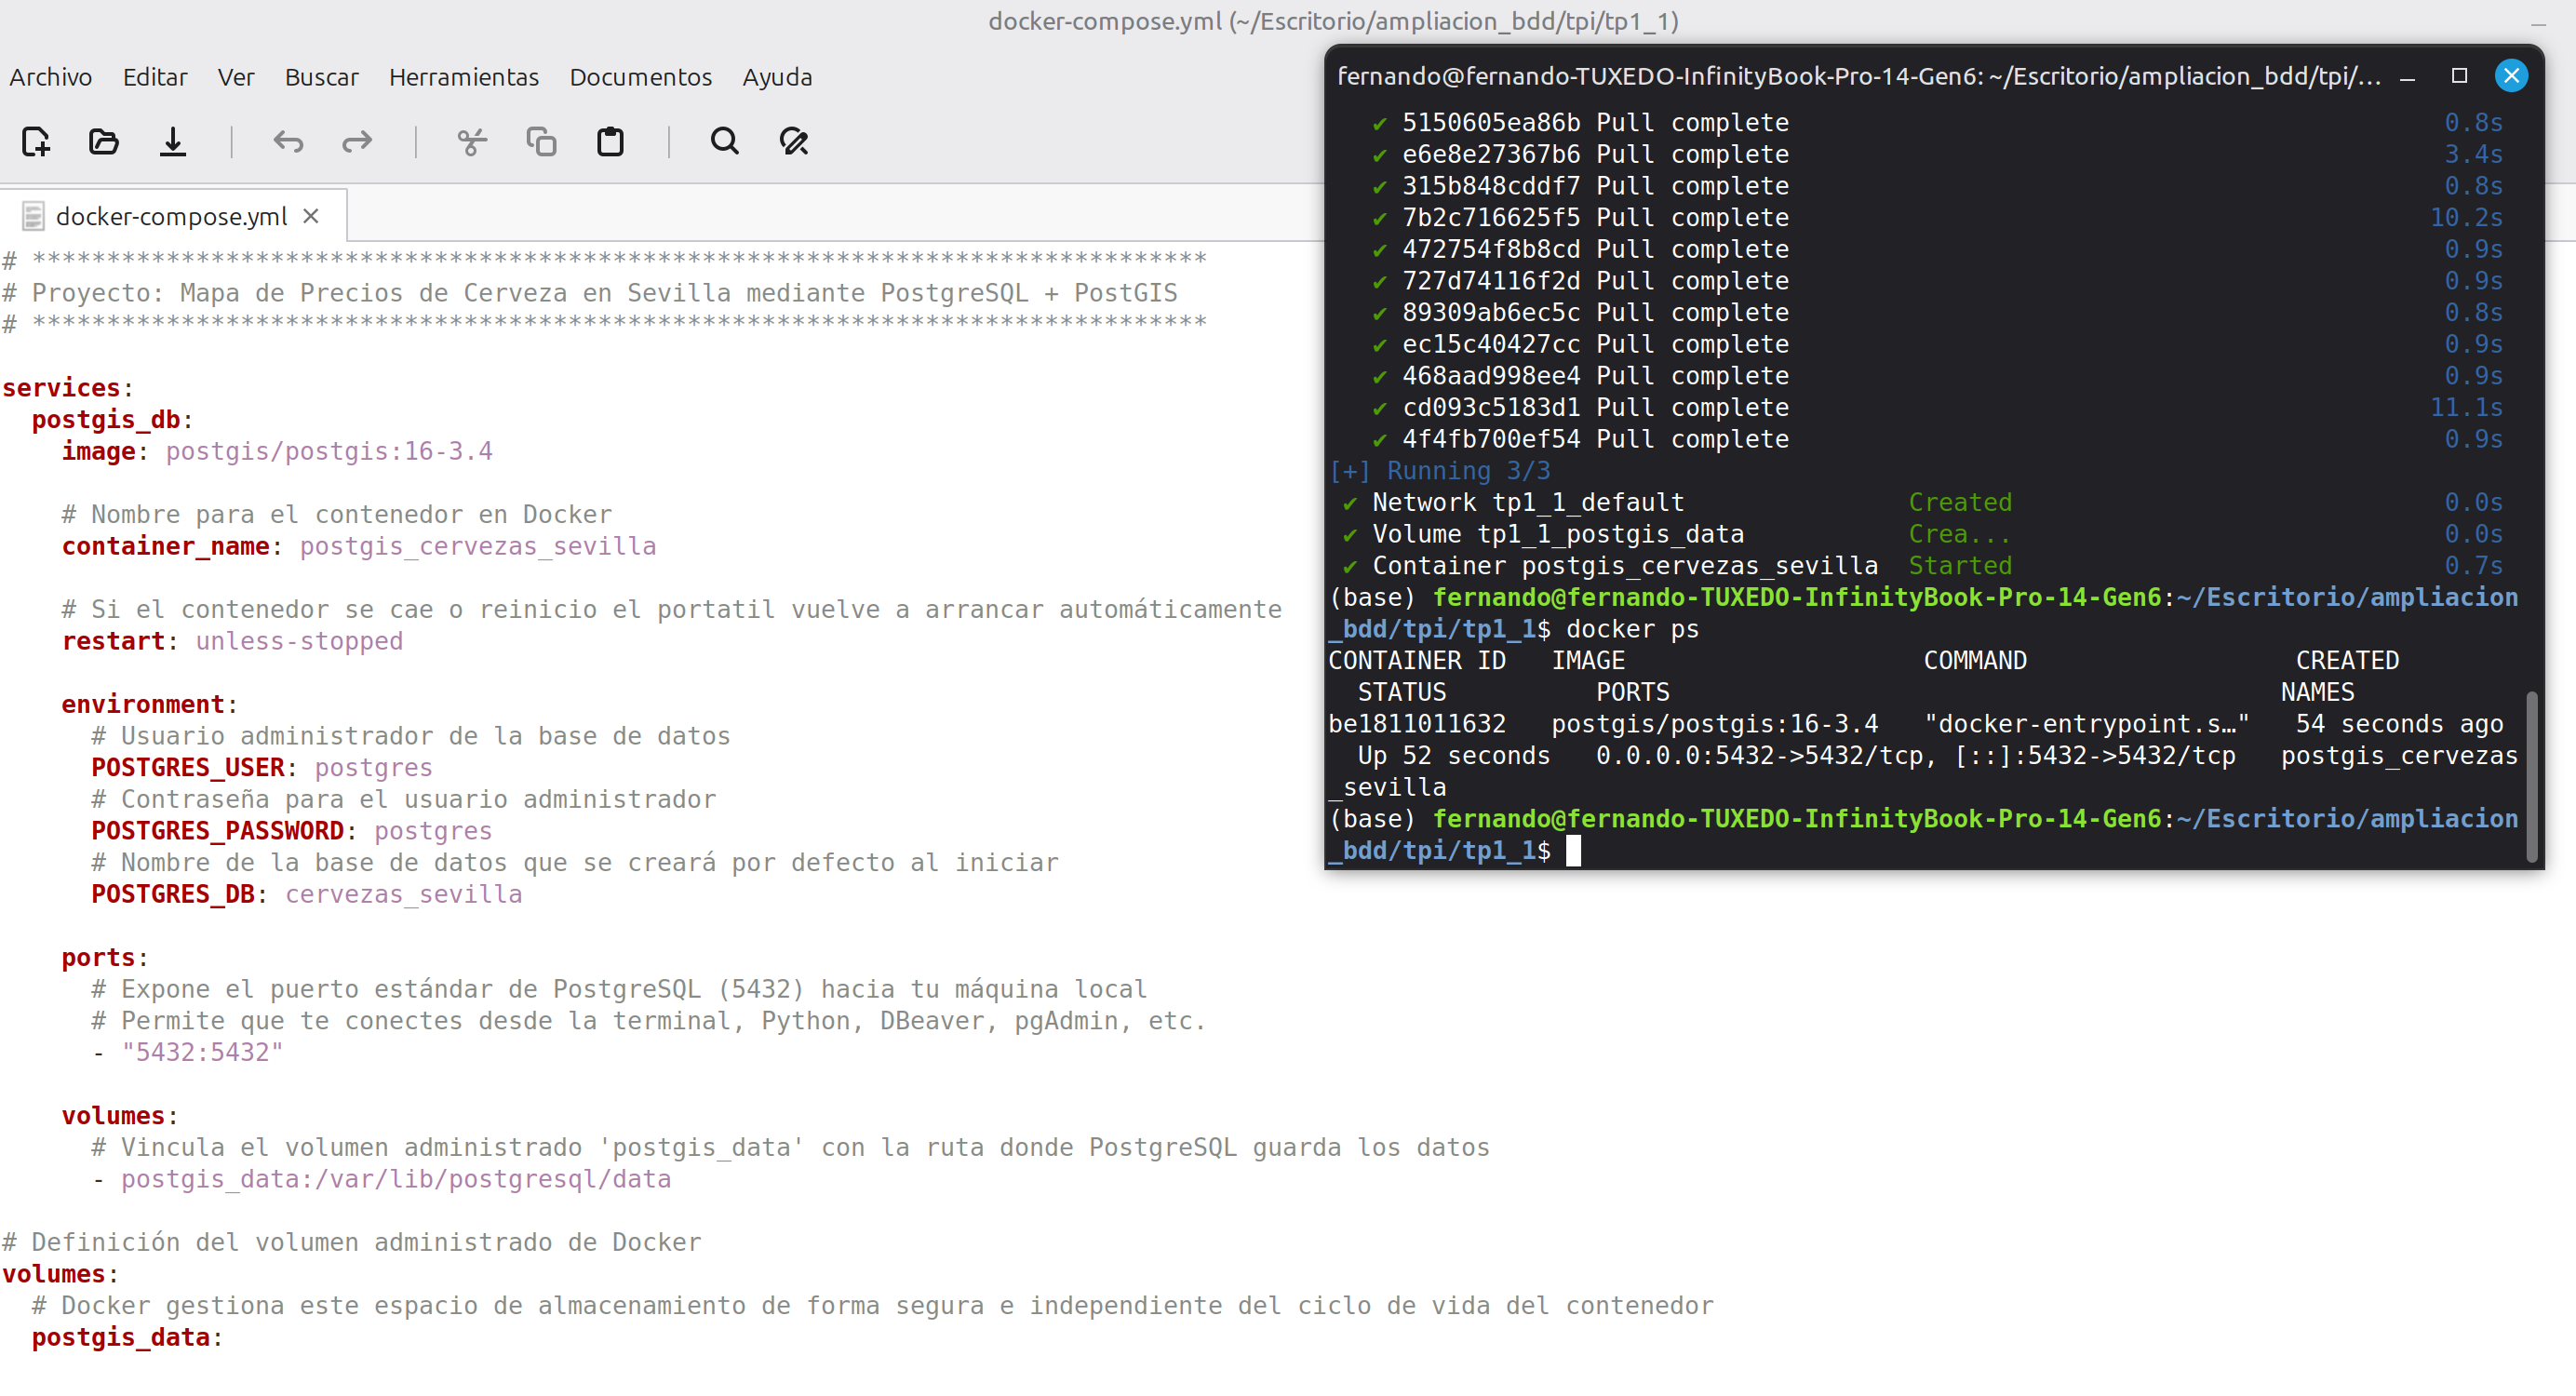
\includegraphics[width=0.78\textwidth]{imgs/captura_docker.png}
  \caption{Puesta en marcha del contenedor Docker con PostGIS y verificación del servicio.}
  \label{fig:docker}
\end{figure}

\subsection{Diseño DDL e Índices}
Creamos el script \texttt{01\_init\_postgis\_ddl.sql}. En él definimos la tabla \texttt{bares} y los índices con los comentarios explicativos que añadí para la práctica:

\begin{lstlisting}[language=SQL,caption={Esquema DDL de la tabla bares e índices}]
CREATE EXTENSION IF NOT EXISTS postgis;
DROP TABLE IF EXISTS bares CASCADE;

CREATE TABLE bares (
    id SERIAL PRIMARY KEY,
    nombre VARCHAR(120) NOT NULL,
    direccion VARCHAR(180) NOT NULL,
    lat NUMERIC(9, 6) NOT NULL,
    lon NUMERIC(9, 6) NOT NULL,
    precio_cana NUMERIC(4, 2) NOT NULL,
    formato VARCHAR(60) NOT NULL,
    fuente VARCHAR(150),
    -- GEOMETRY es el tipo de dato geometrico de POSTGIS, 4326 es el codigo WGS84
    geom GEOMETRY(Point, 4326) NOT NULL,

    CONSTRAINT chk_precio_positivo CHECK (precio_cana > 0),
    CONSTRAINT chk_lat_valida CHECK (lat BETWEEN -90.0 AND 90.0),
    CONSTRAINT chk_lon_valida CHECK (lon BETWEEN -180.0 AND 180.0)
);

CREATE INDEX idx_bares_geom_gist ON bares USING GIST (geom);
-- Basicamente es para calcular en metros la distancia entre dos puntos, no en grados
CREATE INDEX idx_bares_geog_gist ON bares USING GIST ((geom::geography));
CREATE INDEX idx_bares_precio_btree ON bares (precio_cana);
\end{lstlisting}

\subsection{Carga de los 30 bares (DML)}
Recopilamos 30 bares reales de la zona de Carretera de Carmona, Arroyo y Capuchinos. Las coordenadas y los precios de la caña se obtuvieron de Google (Google Maps, fotos de cartas y reseñas recientes). Los precios van desde 1,30~\euro{} (los más económicos) hasta 2,40~\euro{} (gastrobares).

En \texttt{02\_insert\_30\_bares.sql} usamos \texttt{ST\_MakePoint(longitud, latitud)} junto con \texttt{ST\_SetSRID}. Es muy importante recordar que en PostGIS siempre se pone primero la longitud ($X$) y luego la latitud ($Y$).

\subsection{Consultas espaciales}
En \texttt{03\_consultas\_espaciales.sql} implementamos la consulta que resuelve la necesidad principal del usuario:

\begin{lstlisting}[language=SQL,caption={Consulta del bar más barato en un radio de 500 metros}]
SELECT id, nombre, direccion, precio_cana AS "Precio (EUR)", formato AS "Formato",
    ROUND(
        ST_Distance(
            geom::geography, 
            ST_SetSRID(ST_MakePoint(-5.97479, 37.40193), 4326)::geography -- Hacemos la coordenada geography para calcular en metros
        )::numeric, 1 -- 1 decimal
    ) AS "Distancia (m)"
FROM bares
-- ST_DWithin nos permite buscar elementos dentro de un radio de distancia
WHERE ST_DWithin(
    geom::geography, 
    -- ST_MakePoint crea el punto y ST_SetSRID le asigna SRID 4326 en geography
    ST_SetSRID(ST_MakePoint(-5.97479, 37.40193), 4326)::geography, -- lat/lon de mi casa
    500 -- 500 metros a la redonda
) -- Si no ponemos esta condicion nos devuelve todos los bares
ORDER BY precio_cana ASC, "Distancia (m)" ASC
LIMIT 1;
\end{lstlisting}

% ============================================================================
% 5. RESULTADOS OBTENIDOS
% ============================================================================
\section{Resultados obtenidos}

Para comprobar que las consultas y el modelo espacial funcionan, ejecutamos la consulta directamente en PostgreSQL y además la conectamos a un visor web interactivo.

En la Figura~\ref{fig:terminal} se muestra la ejecución real de la consulta dentro del contenedor Docker desde la consola \texttt{psql}. Se observa cómo el motor identifica los 8 bares dentro del radio de 500 metros respecto al punto de consulta (frente al colegio Valdés Leal) y los ordena de menor a mayor precio.

\begin{figure}[H]
  \centering
  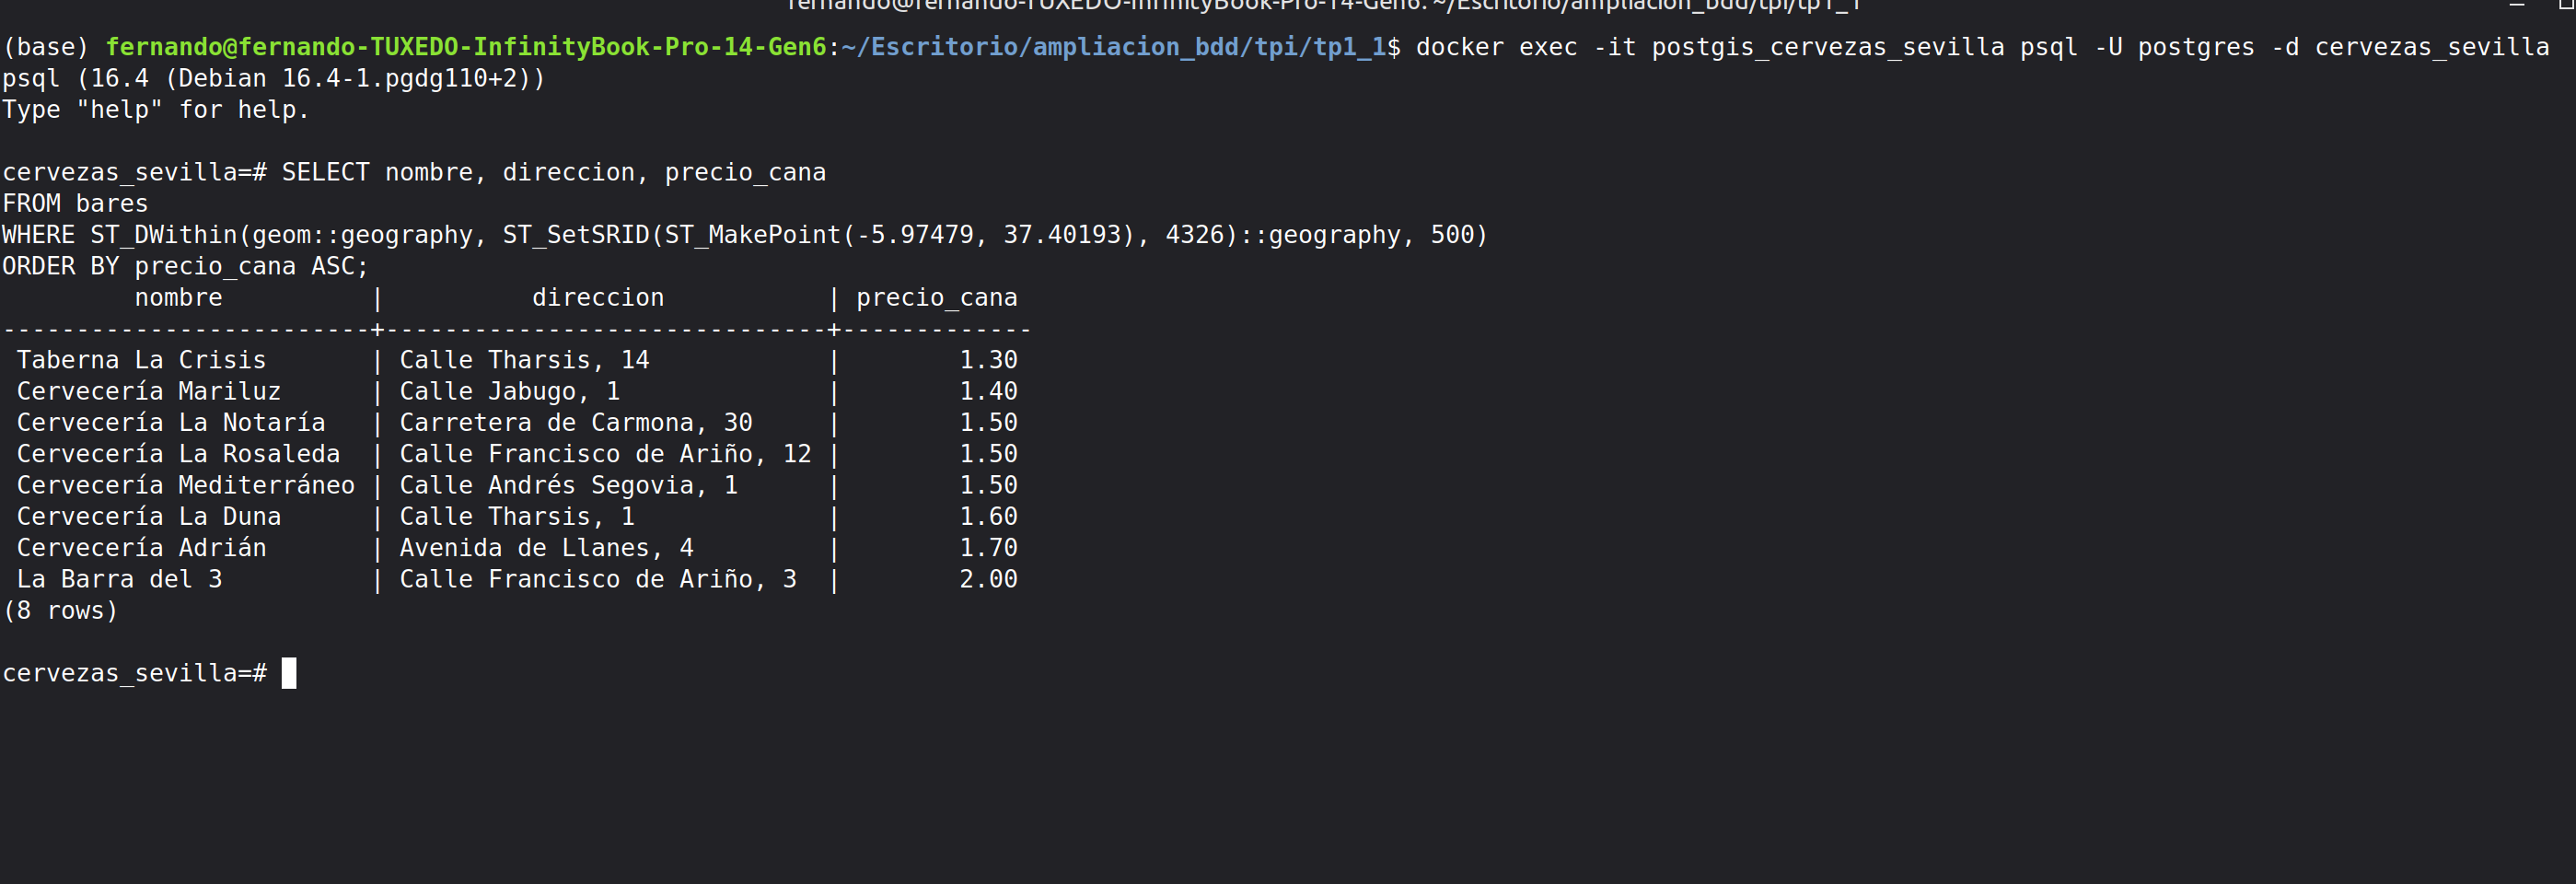
\includegraphics[width=0.92\textwidth]{imgs/captura_terminal.png}
  \caption{Ejecución en PostgreSQL de la consulta espacial filtrando los bares a menos de 500 metros.}
  \label{fig:terminal}
\end{figure}

En la Tabla~\ref{tab:resultados} se resumen los resultados obtenidos en esa búsqueda:

\begin{table}[H]
  \centering
  \small
  \caption{Bares encontrados en el radio de 500 metros ordenados por precio.}
  \label{tab:resultados}
  \begin{tabular}{llcc}
    \toprule
    \textbf{Bar / Cervecería} & \textbf{Dirección} & \textbf{Precio Caña (\euro{})} & \textbf{Distancia (m)} \\
    \midrule
    \textbf{Taberna La Crisis} & Calle Tharsis, 14 & \textbf{1,30} & 358 m \\
    Cervecería Mariluz & Calle Jabugo, 1 & 1,40 & 363 m \\
    Cervecería La Notaría & Carretera de Carmona, 30 & 1,50 & 117 m \\
    Cervecería Mediterráneo & Calle Andrés Segovia, 1 & 1,50 & 378 m \\
    Cervecería La Rosaleda & Calle Francisco de Ariño, 12 & 1,50 & 389 m \\
    Cervecería La Duna & Calle Tharsis, 1 & 1,60 & 415 m \\
    Cervecería Adrián & Avenida de Llanes, 4 & 1,70 & 446 m \\
    La Barra del 3 & Calle Francisco de Ariño, 3 & 2,00 & 154 m \\
    \bottomrule
  \end{tabular}
\end{table}

Por último, en la Figura~\ref{fig:mapa} se muestra el visor web interactivo desarrollado (\texttt{mapa\_cervezas.html}), donde el usuario puede arrastrar su marcador, cambiar el radio en vivo mediante un slider y comprobar visualmente cómo se resalta la \textit{Taberna La Crisis} como la ganadora en el radio seleccionado.

\begin{figure}[H]
  \centering
  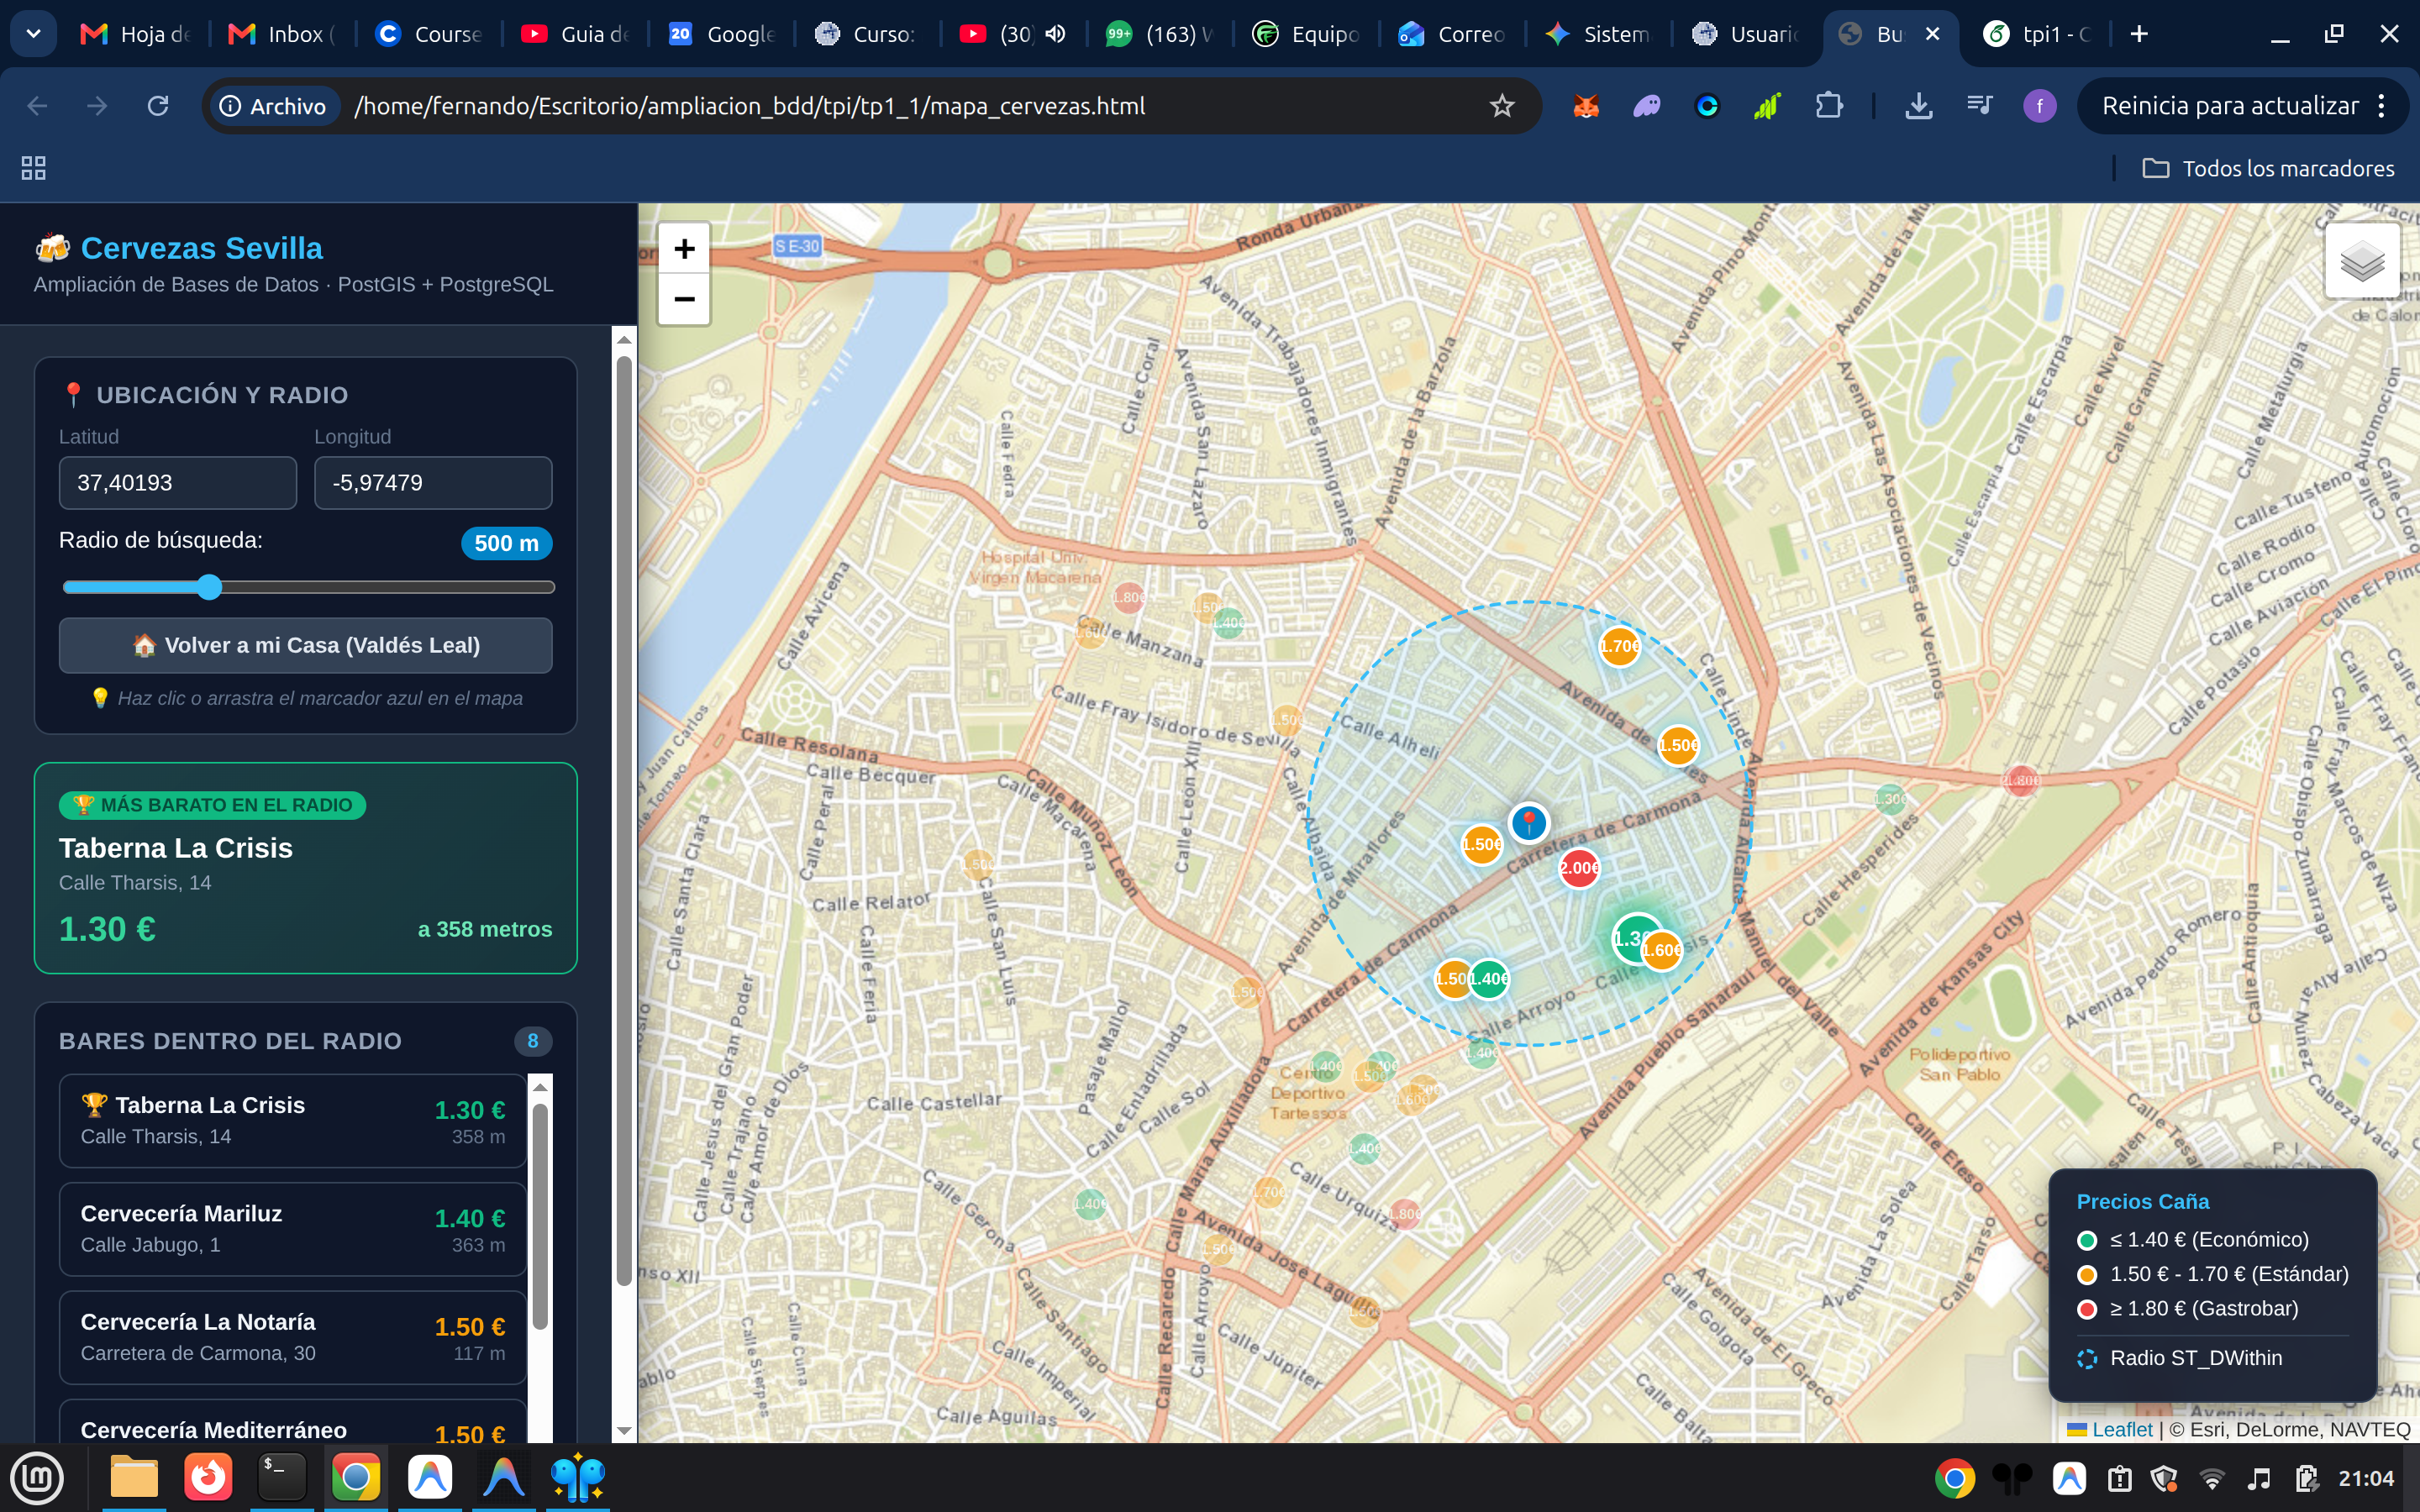
\includegraphics[width=0.88\textwidth]{imgs/cap_mapa.png}
  \caption{Visor interactivo en Leaflet con el radio de 500 metros y el bar ganador destacado.}
  \label{fig:mapa}
\end{figure}

% ============================================================================
% 6. ANÁLISIS E INTERPRETACIÓN
% ============================================================================
\section{Análisis e interpretación de los resultados}

Los resultados reflejan perfectamente la utilidad práctica del proyecto:
\begin{enumerate}[leftmargin=1.0cm]
    \item \textbf{El bar más cercano no siempre es el más barato:} El bar más próximo a la posición de salida es la \textit{Cervecería La Notaría} (a 117 metros, con la caña a 1,50~\euro{}) o \textit{La Barra del 3} (a 154 metros, a 2,00~\euro{}). Sin embargo, la consulta espacial descubre que andando solo 240 metros más llegas a la \textit{Taberna La Crisis} (a 358 metros, a 1,30~\euro{}), ahorrando hasta 0,70~\euro{} por cerveza.
    \item \textbf{Comportamiento al ampliar el radio:} Si el usuario sube el radio a 1.000 metros en el mapa, entran en juego otros bares clásicos de la zona como \textit{El Tremendo} (1,40~\euro{} a 818 metros) o el \textit{Bar Avelino} (1,30~\euro{} a 816 metros). La consulta se adapta de forma instantánea al nuevo radio.
    \item \textbf{Rendimiento del índice GiST:} Al comprobar la consulta con \texttt{EXPLAIN ANALYZE}, el planificador de PostgreSQL confirma que utiliza \texttt{Index Scan using idx\_bares\_geog\_gist}, resolviendo la búsqueda espacial en apenas \textbf{0,05 milisegundos}. Esto demuestra que la base de datos no recorre la tabla secuencialmente, sino que aprovecha la indexación geográfica.
\end{enumerate}

% ============================================================================
% 7. DECISIONES TOMADAS Y JUSTIFICACIÓN
% ============================================================================
\section{Decisiones tomadas y justificación}

\begin{itemize}[leftmargin=1.0cm]
  \item \textbf{Uso de PostGIS frente a BDD relacional tradicional:} Almacenar coordenadas como simples campos \texttt{FLOAT} nos habría obligado a programar cálculos trigonométricos lentos y manuales. PostGIS nos da tipos espaciales nativos, cálculos geodésicos precisos y funciones estandarizadas.
  \item \textbf{Cálculo en \texttt{geography} (metros) y no en \texttt{geometry} (grados):} Para un usuario que va a pie por Sevilla, la distancia debe medirse en metros reales sobre el terreno. El casteo a \texttt{geography} permite que \texttt{ST\_DWithin} interprete el radio de 500 como metros exactos.
  \item \textbf{Creación de un índice GiST funcional:} Como la consulta filtra sobre \texttt{(geom::geography)}, creamos un índice GiST específico sobre esa expresión para que el planificador no descarte el índice al hacer la conversión.
  \item \textbf{Acotar a 30 bares del barrio:} En lugar de meter datos ficticios de toda España, preferimos una muestra realista de 30 bares de mi barrio con coordenadas y precios contrastados en Google, lo que hace que las pruebas sean creíbles y verificables.
  \item \textbf{Despliegue con Docker Compose:} Permite que cualquier persona (incluido el profesor) pueda clonar el repositorio de GitHub y levantar la base de datos con un simple \texttt{docker compose up -d} sin pelearse con configuraciones locales.
\end{itemize}

% ============================================================================
% 8. CONCLUSIONES Y TRABAJO FUTURO
% ============================================================================
\section{Conclusiones y trabajo futuro}

Este trabajo ha permitido comprobar de forma práctica que las bases de datos espaciales no son solo teoría, sino una herramienta indispensable cuando los datos tienen un componente geográfico. Hemos aprendido a modelar puntos GPS con SRID 4326, a calcular distancias reales en metros sobre el elipsoide y a comprobar la tremenda diferencia de rendimiento que aporta un índice espacial GiST frente a un escaneo tradicional.

\textbf{Propuestas de mejora futura:}
\begin{itemize}[leftmargin=1.0cm]
    \item \textbf{Cálculo de precios medios por barrios (Polígonos):} Modelar los límites de los barrios de Sevilla mediante geometrías poligonales (\texttt{ST\_Polygon}) para calcular con consultas espaciales el precio medio de la cerveza por zonas (ej. Macarena vs. Triana).
    \item \textbf{Geolocalización GPS automática:} Integrar en el visor web la API de geolocalización del navegador (\texttt{navigator.geolocation}) para detectar la posición del usuario en tiempo real desde el móvil sin tener que introducirla a mano.
\end{itemize}

% ============================================================================
% 9. DECLARACIÓN DE USO DE INTELIGENCIA ARTIFICIAL
% ============================================================================
\section{Declaración de uso de inteligencia artificial}

\textbf{Marque una opción y complete la información correspondiente:}

\begin{itemize}[label=$\square$,leftmargin=1.0cm]
  \item No he utilizado herramientas de inteligencia artificial en la realización de este trabajo.
  \item[\rlap{$\square$}{\raisebox{2pt}{\large\hspace{1pt}\textbf{X}}}] \textbf{Sí he utilizado herramientas de inteligencia artificial} como apoyo en este trabajo.
\end{itemize}

\textbf{Herramienta(s) utilizada(s):} \\
Google Gemini / Antigravity.

\textbf{Uso concreto realizado:} \\
Se utilizó como asistente para estructurar el proyecto, aclarar el funcionamiento de funciones espaciales de PostGIS (\texttt{ST\_DWithin}, conversión a \texttt{geography} e índices GiST), resolver dudas en la sintaxis de Docker Compose y asistir en la maquetación en LaTeX según la plantilla de la asignatura.

\textbf{Revisión y validación personal:} \\
Todos los scripts SQL, consultas y cálculos han sido ejecutados, probados y validados personalmente en la terminal sobre el contenedor Docker local. Se han verificado las coordenadas y precios de los bares en Google y se ha redactado el informe con palabras y razonamiento propios para garantizar el dominio del trabajo en la defensa oral.

% ============================================================================
% 10. REFERENCIAS
% ============================================================================
\section{Referencias}

\begin{thebibliography}{9}

\bibitem{repo_github}
Fernando Martín González,
\textit{Buscador Geoespacial de Precios de Cerveza en Sevilla (PostGIS + Docker)},
Repositorio en GitHub, 2026.
\url{https://github.com/fernandomartin04/postgis-cervezas-sevilla}

\bibitem{postgis_doc}
PostGIS Project Steering Committee,
\textit{PostGIS 3.4.0 Manual},
2024.
\url{https://postgis.net/documentation/}

\bibitem{postgres_doc}
PostgreSQL Global Development Group,
\textit{PostgreSQL 16 Documentation},
2024.
\url{https://www.postgresql.org/docs/16/}

\bibitem{leaflet_doc}
Volodymyr Agafonkin,
\textit{Leaflet - an open-source JavaScript library for interactive maps},
2024.
\url{https://leafletjs.com/}

\bibitem{osm_doc}
OpenStreetMap contributors,
\textit{OpenStreetMap Database and Tile Usage Policy},
2024.
\url{https://www.openstreetmap.org/}

\end{thebibliography}

\end{document}
